\documentclass[12pt,a4paper]{article}
\usepackage[utf8]{vietnam}
\usepackage{amsmath,amssymb}
\usepackage{geometry}
\geometry{top=1.5cm,bottom=1.2cm,left=1.4cm,right=1.4cm,headheight=28pt,headsep=12pt,footskip=18pt}
\usepackage{tikz}
\usepackage{xcolor}
\usepackage{enumerate}
\usepackage{graphicx}
\usepackage[version=4]{mhchem}
\usepackage{fancyhdr}
\usepackage{ex_test}

\renewcommand{\baselinestretch}{0.96}
\setlength{\parskip}{0pt}

\definecolor{hfRed}{RGB}{211,47,47}
\definecolor{hfGreen}{RGB}{139,195,144}

\pagestyle{fancy}
\fancyhf{}
\fancyhead[L]{\small\itshape\color{hfRed} Tài liệu lưu hành nội bộ}
\fancyhead[R]{\small\itshape\color{hfRed} Thầy \textbf{TRẦN VĂN THẠNH} - 0777.470.803}
\renewcommand{\headrulewidth}{0.8pt}
\renewcommand{\headrule}{\hbox to\headwidth{\color{hfGreen}\leaders\hrule height \headrulewidth\hfill}}

\fancyfoot[L]{\small\itshape\color{hfRed} CS1: 6/15 Nguyễn Hoàng, P. Kim Long, TP Huế \quad|\quad CS2: 24 Đặng Thái Thân, TP Huế}
\fancyfoot[R]{\small\bfseries\color{hfRed} Trang \thepage}
\renewcommand{\footrulewidth}{0.8pt}
\renewcommand{\footrule}{\hbox to\headwidth{\color{hfGreen}\leaders\hrule height \footrulewidth\hfill}}

\fancypagestyle{firstpage}{
  \fancyhf{}
  \renewcommand{\headrulewidth}{0pt}
  \fancyfoot[L]{\small\itshape\color{hfRed} CS1: 6/15 Nguyễn Hoàng, P. Kim Long, TP Huế \quad|\quad CS2: 24 Đặng Thái Thân, TP Huế}
  \fancyfoot[R]{\small\bfseries\color{hfRed} Trang \thepage}
  \renewcommand{\footrulewidth}{0.8pt}
  \renewcommand{\footrule}{\hbox to\headwidth{\color{hfGreen}\leaders\hrule height \footrulewidth\hfill}}
}

\begin{document}
\thispagestyle{firstpage}

\noindent
\begin{minipage}[t]{0.44\textwidth}
	\centering\fontsize{10pt}{12pt}\selectfont
	\textbf{SỞ GIÁO DỤC VÀ ĐÀO TẠO THỪA THIÊN HUẾ}\\
	\textbf{ĐỀ CHÍNH THỨC}\\
	\textit{(Đề thi có 04 trang)}
\end{minipage}\hfill
\begin{minipage}[t]{0.54\textwidth}
	\centering\small
	\textbf{ĐỀ KIỂM TRA ĐỊNH KỲ CHƯƠNG 2 (NITROGEN -- SULFUR)}\\
	\textbf{MÔN: HOÁ HỌC -- LỚP 11}\\
	\textit{Thời gian làm bài: 45 phút (không kể thời gian phát đề)}\\
	\fbox{\textbf{MÃ ĐỀ: 106}}
\end{minipage}

\smallskip
\noindent\hrulefill
\smallskip

\noindent\textbf{Họ, tên thí sinh:} \dotfill\ \textbf{Lớp:} \dotfill\ \textbf{Số báo danh:} \dotfill

\smallskip
\noindent\textit{(Cho biết nguyên tử khối: H = 1; C = 12; N = 14; O = 16; Na = 23; Mg = 24; Al = 27; S = 32; Cl = 35,5; K = 39; Ca = 40; Fe = 56; Cu = 64; Zn = 65; Ag = 108; Ba = 137; Au = 197).}
\smallskip

\noindent\textbf{\large PHẦN I. Câu trắc nghiệm nhiều phương án lựa chọn.}
\textit{Thí sinh trả lời từ câu 1 đến câu 18. Mỗi câu hỏi thí sinh chỉ chọn một phương án.}
\vspace{0.2cm}

\Opensolutionfile{ans}[ans-hoa11-de06hs]

\begin{ex}
\textbf{(SBT - CTST)} Ở trạng thái tự nhiên, nitrogen
\choice
{\True tồn tại ở dạng đơn chất và hợp chất}
{chỉ tồn tại ở dạng đơn chất}
{chỉ tồn tại ở dạng hợp chất}
{tự do chiếm khoảng 20\% thể tích không khí}

\end{ex}

\begin{ex}
\textbf{(SBT - KNTT)} Trong phương pháp Ostwald, ammonia bị oxi hóa bởi oxygen không khí tạo thành sản phẩm chính là
\choice
{\True $\ce{NO}$}
{$\ce{N2}$}
{$\ce{N2O}$}
{$\ce{NO2}$}

\end{ex}

\begin{ex}
\textbf{[KNTT - SBT]} Cho các chất khí sau: $\ce{H2S, NO, NO2, SO2}$. Số khí gây ô nhiễm môi trường khi phát thải vào không khí là
\choice
{1}
{\True 4}
{3}
{2}

\end{ex}

\begin{ex}
\textbf{(SBT - KNTT)} Oxide của nitrogen được tạo thành khi nguyên tố nitrogen trong nhiên liệu hoặc sinh khối kết hợp với oxygen dư thừa trong không khí được gọi là
\choice
{$\ce{NO_x}$ tức thời}
{$\ce{NO_x}$ nhiệt}
{\True $\ce{NO_x}$ nhiên liệu}
{$\ce{NO_x}$ tự nhiên}

\end{ex}

\begin{ex}
\textbf{[CD - SBT]} Phát biểu nào sau đây về đơn chất nitrogen ($\ce{N2}$) là \textbf{không} đúng?
\choice
{\True Dù phân tử $\ce{N2}$ có tính kém hoạt động hóa học, nhưng vẫn hoạt động hóa học mạnh hơn chlorine, $\ce{Cl2}$}
{Đơn chất nitrogen không phản ứng với hydrogen, oxygen ở điều kiện thường}
{Do có nhiệt độ rất thấp nên nitrogen lỏng được sử dụng bảo quản một số loại mẫu vật}
{Trong bầu khí quyển, khi có sấm chớp, khí nitrogen tạo các nitrogen oxide, là một nguyên nhân làm cho nước mưa có tính acid}

\end{ex}

\begin{ex}
\textbf{(SBT - KNTT)} Ở điều kiện thích hợp, sulfur dioxide đóng vai trò là chất oxi hoá khi tham gia phản ứng với chất nào sau đây?
\choice
{$\ce{NO2}$}
{\True $\ce{H2S}$}
{$\ce{NaOH}$}
{$\ce{Ca(OH)2}$}

\end{ex}

\begin{ex}
\textbf{(SBT - CTST)} Điều nào sau đây đúng về tính chất hóa học của dung dịch $\ce{H2SO4}$ đặc?
\choice
{Dung dịch $\ce{H2SO4}$ đặc có tính khử mạnh}
{\True Dung dịch $\ce{H2SO4}$ đặc có tính oxi hóa mạnh}
{Dung dịch $\ce{H2SO4}$ đặc vừa có tính khử, vừa có tính oxi hóa}
{Dung dịch $\ce{H2SO4}$ đặc không có tính khử, không có tính oxi hóa}

\end{ex}

\begin{ex}
\textbf{(SBT - KNTT)} Xét phản ứng trong quá trình tạo ra $\ce{NO_x}$ nhiệt:
\[\ce{N2(g) + O2(g) -> 2NO(g)} \quad \Delta_r H^\circ_{298} = 180{,}6\text{ kJ}\]
Nhiệt tạo thành chuẩn của $\ce{NO(g)}$ là
\choice
{$180{,}6\text{ kJ/mol}$}
{$-180{,}6\text{ kJ/mol}$}
{$-90{,}3\text{ kJ/mol}$}
{\True $90{,}3\text{ kJ/mol}$}

\end{ex}

\begin{ex}
\textbf{(SBT - KNTT)} Xét cân bằng hóa học: $\ce{N2(g) + 3H2(g) <=> 2NH3(g)} \quad \Delta_r H^\circ_{298} < 0$.\\
Hiệu suất phản ứng khi hệ đạt cân bằng ở nhiệt độ $400^\circ\text{C}$ và $500^\circ\text{C}$ lần lượt bằng $x\%$ và $y\%$. Mối quan hệ giữa $x$ và $y$ là
\choice
{$x < y$}
{$x = y$}
{\True $x > y$}
{$5x = 4y$}

\end{ex}

\begin{ex}
Muốn cho cân bằng của phản ứng tổng hợp ammonia chuyển dịch sang phải cần đồng thời:
\[\ce{N2 + 3H2 <=> 2NH3} \quad \Delta_r H^\circ_{298} < 0\]
\choice
{Tăng áp suất và tăng nhiệt độ}
{\True Tăng áp suất và giảm nhiệt độ}
{Giảm áp suất và giảm nhiệt độ}
{Giảm áp suất và tăng nhiệt độ}

\end{ex}

\begin{ex}
Hợp chất vô cơ X có các tính chất: X tinh khiết là chất lỏng không màu, bốc khói mạnh trong không khí ẩm; dung dịch X đặc để lâu có màu vàng; tan tốt trong nước; có tính oxi hóa mạnh. Chất X là
\choice
{$\ce{H3PO4}$}
{\True $\ce{HNO3}$}
{$\ce{H2SO4}$}
{$\ce{HCl}$}

\end{ex}

\begin{ex}
\textbf{[KNTT - SBT]} Cho cân bằng hóa học sau: $\ce{2SO2(g) + O2(g) <=> 2SO3(g)} \quad \Delta_r H^\circ_{298} < 0$.\\
Khi tăng nhiệt độ thì
\choice
{Tổng số mol khí trong hệ giảm}
{Hiệu suất phản ứng tăng}
{\True Cân bằng chuyển dịch theo chiều nghịch}
{Nồng độ khí sản phẩm tăng}

\end{ex}

\begin{ex}
\textbf{[KNTT - SBT]} Trong công nghiệp sản xuất sulfuric acid, hai nguồn nguyên liệu được khai thác từ mỏ để cung cấp nguyên tố lưu huỳnh là
\choice
{$\ce{ZnS, PbS}$}
{$\ce{H2S, SO2}$}
{$\ce{CaSO4, BaSO4}$}
{\True $\ce{S, FeS2}$}

\end{ex}

\begin{ex}
Nếu ta dẫn khí $\ce{SO2}$ từ từ đến dư vào dung dịch bromine sẽ có phản ứng hóa học xảy ra kèm hiện tượng gì sau đây?
\choice
{Dung dịch không đổi màu}
{Dung dịch bị vẩn đục do tạo kết tủa và kết tủa không tan}
{Dung dịch sẽ có màu đỏ nâu đậm dần lên hơn lúc ban đầu}
{\True Dung dịch sẽ nhạt màu đỏ nâu rồi mất hẳn màu}

\end{ex}

\begin{ex}
Hậu quả chính của hiện tượng phú dưỡng đối với môi trường nước là gì?
\choice
{Làm tăng độ trong suốt của nước và giúp cải thiện hệ sinh thái thủy sinh}
{\True Làm giảm lượng oxygen hòa tan trong nước, gây ra hiện tượng cá chết hàng loạt và phá hủy hệ sinh thái}
{Tăng nồng độ oxygen hòa tan trong nước, giúp thủy sinh vật phát triển mạnh mẽ hơn}
{Giảm sự phát triển của vi sinh vật trong nước}

\end{ex}

\begin{ex}
Loại khí nào dưới đây là nguyên nhân chính gây ra mưa acid?
\choice
{Khí $\ce{CO2}$}
{Khí $\ce{O2}$}
{\True Khí $\ce{SO2}$ và $\ce{NO_x}$}
{Khí $\ce{CH4}$}

\end{ex}

\begin{ex}
Khu vực nào có nguy cơ bị ảnh hưởng nghiêm trọng bởi mưa acid?
\choice
{Những khu vực có nhiều cây cối và hệ sinh thái phong phú}
{\True Những khu vực gần các nhà máy điện, nhà máy công nghiệp và giao thông dày đặc}
{Những khu vực có độ cao lớn}
{Những khu vực gần biển}

\end{ex}

\begin{ex}
Cho các phát biểu sau:
\begin{enumerate}[(1)]
	\item Phương pháp tiếp xúc gồm ba công đoạn chính sản xuất: $\ce{SO2, SO3, H2SO4}$.
	\item Ở giai đoạn tạo ra $\ce{SO3}$, người ta chọn điều kiện phản ứng ở nhiệt độ thấp.
	\item Nhờ có chất xúc tác nên phản ứng giữa $\ce{SO2}$ và $\ce{O2}$ ưu tiên diễn ra theo chiều thuận.
	\item Khí sulfur trioxide đi từ dưới lên đỉnh tháp, sulfuric acid đặc chảy từ đỉnh tháp xuống dưới.
	\item Tương tác van der Waals giữa các phân tử nitrogen với nước rất yếu nên ít tan trong nước.
	\item Phân tử nitrogen nặng hơn không khí và không phân cực.
	\item Nitrogen lỏng ở nhiệt độ thấp, $-196^\circ\text{C}$ và có tính trơ.
\end{enumerate}
Số phát biểu đúng là
\choice
{3}
{\True 4}
{5}
{6}

\end{ex}

\Closesolutionfile{ans}

\vspace{0.3cm}
\noindent\textbf{\large PHẦN II. Câu trắc nghiệm đúng sai.}
\textit{Thí sinh trả lời từ câu 1 đến câu 4. Trong mỗi ý a), b), c), d) ở mỗi câu, thí sinh chọn đúng hoặc sai.}
\vspace{0.2cm}

\begin{ex}
Hợp chất có công thức hóa học $\ce{NH4NO3}$ được giới chức quốc gia Lebanon xác định là nguyên nhân gây ra vụ nổ thảm khốc ở thủ đô Beirut vào ngày 04/08/2020. Tia lửa hàn trong quá trình sửa chữa nhà kho có thể đã làm 2 750 tấn $\ce{NH4NO3}$ cất trữ phát nổ, phá hủy nhiều nhà cửa, dẫn đến nhiều người thiệt mạng.
\[\ce{NH4NO3 ->[t^\circ] N2O + 2H2O} \quad \Delta_r H^\circ_{298} = -35{,}9\text{ kJ}\]
\choiceTF
{Ammonium nitrate khi ở nhiệt độ cao bị phân hủy thành khí $\ce{N2O}$ và hơi nước, là một phản ứng thu nhiệt và năng lượng lớn}
{\True Khi phản ứng nổ xảy ra, năng lượng được giải phóng một cách đột ngột dưới áp lực rất cao, tăng nhanh, còn được gọi là sóng nổ hoặc sóng xung kích}
{\True Sóng xung kích gây ra thiệt hại lớn cho môi trường xung quanh. Ammonium nitrate có thể tự phân hủy qua thời gian}
{\True Tia lửa hàn trong quá trình sửa chữa nhà kho đã khơi mào phản ứng phân hủy ammonium nitrate gây nổ}

\end{ex}

\begin{ex}
Nguồn nào sau đây phát sinh oxide của nitrogen trong không khí?
\choiceTF
{\True Đốt cháy các nhiên liệu hóa thạch}
{\True Quá trình sản xuất và sử dụng nitric acid}
{\True Trong khí quyển khi có sấm sét}
{Quá trình quang hợp của cây xanh}

\end{ex}

\begin{ex}
Sulfur dioxide là một chất có nhiều ứng dụng trong công nghiệp (dùng để sản xuất sulfuric acid, tẩy trắng bột giấy công nghiệp giấy, tẩy trắng dung dịch đường trong sản xuất đường tinh luyện,...) và giúp ngăn cản sự phát triển của một số loại vi khuẩn và nấm gây hại cho thực phẩm. Ở áp suất 1 bar và nhiệt độ $25^\circ\text{C}$, phản ứng giữa 1 mol sulfur với oxygen xảy ra theo phương trình:
\[\ce{S(s) + O2(g) -> SO2(g)}\]
và tỏa ra một lượng nhiệt là $296{,}9\text{ kJ}$.
\begin{center}
	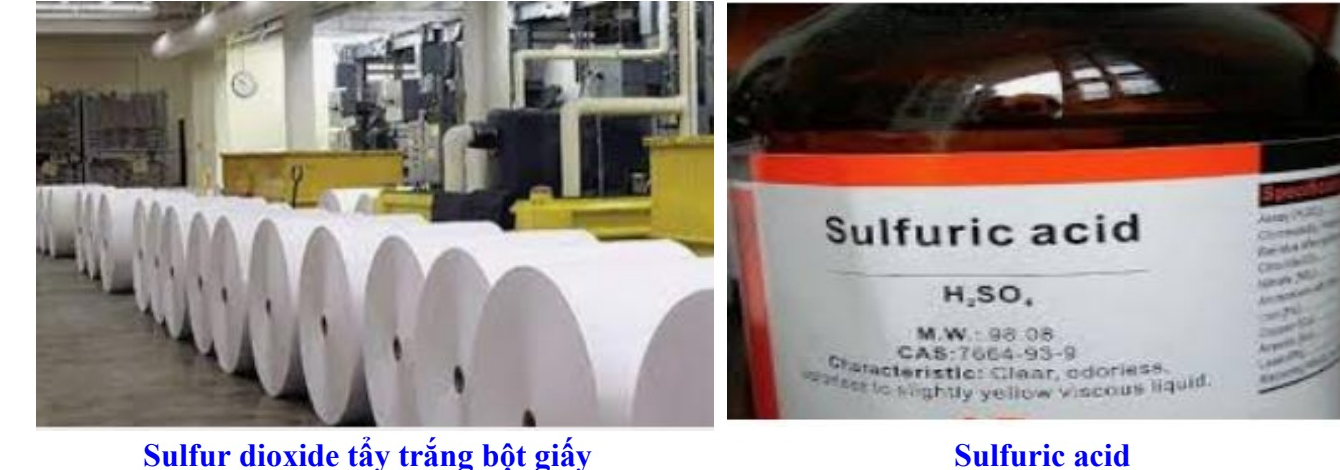
\includegraphics[width=0.75\textwidth]{images_crop_hoa11_de06/cau3_p2_so2_ungdung.png}
\end{center}
\choiceTF
{Biến thiên enthalpy chuẩn của phản ứng là $296{,}9\text{ kJ}$}
{\True Enthalpy tạo thành chuẩn của sulfur dioxide bằng $-296{,}9\text{ kJ}\cdot\text{mol}^{-1}$}
{\True Sulfur dioxide vừa có thể là chất khử vừa có thể là chất oxi hóa, tùy thuộc vào phản ứng mà nó tham gia}
{\True 0,5 mol sulfur tác dụng hết oxygen giải phóng $148{,}45\text{ kJ}$ năng lượng dưới dạng nhiệt}

\end{ex}

\begin{ex}
Sulfuric acid có hoạt tính hóa học rất mạnh:
\choiceTF
{Nhôm (aluminum) bị thụ động trong dung dịch $\ce{H2SO4}$ loãng nguội}
{\True Hỗn hợp gồm $\ce{Cu}$ và $\ce{Fe2O3}$ có tỉ lệ mol 1:1 tan hết trong dung dịch $\ce{H2SO4}$ loãng}
{\True Khi cho $\ce{H2SO4}$ đặc vào đường kính trắng ($\ce{C12H22O11}$), khí thoát ra làm mất màu dung dịch $\ce{KMnO4}$}
{$\ce{H2SO4}$ đặc có thể dùng để làm khô các khí $\ce{CO2, Cl2, N2, H2S}$}

\end{ex}

\vspace{0.3cm}
\noindent\textbf{\large PHẦN III. Câu trắc nghiệm yêu cầu trả lời ngắn.}
\textit{Thí sinh trả lời từ câu 1 đến câu 6.}
\vspace{0.2cm}

\begin{ex}
Cho các chất sau: $\ce{H2SO4, CO2, CO, N2, NH3}$. Số chất tan tốt trong nước ở nhiệt độ thường là bao nhiêu?

\vspace{1.0cm}

\end{ex}

\begin{ex}
Cho các phản ứng:
\begin{enumerate}[(a)]
	\item $\ce{S + O2 ->[t^\circ] SO2}$
	\item $\ce{S + 3F2 -> SF6}$
	\item $\ce{Hg + S -> HgS}$
	\item $\ce{H2 + S ->[t^\circ] H2S}$
\end{enumerate}
Số phản ứng trong đó sulfur đơn chất đóng vai trò chất oxi hóa là bao nhiêu?

\vspace{1.0cm}

\end{ex}

\begin{ex}
Cho các chất: $\ce{HCl}$ (aq hoặc khí), $\ce{O2}\ (t^\circ)$, $\ce{AlCl3}$ (aq), $\ce{H2SO4}$ (aq), $\ce{NaOH}$ (aq), $\ce{Na2CO3}$ (aq), $\ce{CuO}$. Có bao nhiêu chất phản ứng được với $\ce{NH3}$?

\vspace{1.5cm}

\end{ex}

\begin{ex}
Cho hỗn hợp khí (X) gồm $\ce{N2, H2, NH3}$ có tỉ khối so với khí hydrogen là 8. Dẫn hỗn hợp khí (X) đi qua dung dịch $\ce{H2SO4}$ đặc, dư thì thể tích khí còn lại một nửa. Thành phần \% theo thể tích của $\ce{NH3}$ trong hỗn hợp (X) là $x\%$. Xác định giá trị $x$.

\vspace{1.5cm}

\end{ex}

\begin{ex}
Tại nhiều làng nghề thủ công mĩ nghệ, sulfur dioxide được dùng là chất chống mốc cho các sản phẩm mây tre đan. Trong một ngày, một làng nghề đốt cháy $20\text{ kg}$ sulfur để tạo thành sulfur dioxide. Giả thiết có 20\% lượng khí $\ce{SO2}$ trên bay vào khí quyển và chuyển hoá hết thành $\ce{H2SO4}$ trong nước mưa theo sơ đồ:
\[\ce{SO2 ->[+O2, xt] SO3 ->[+H2O] H2SO4}\]
Thể tích nước mưa là $x$ nghìn $\text{m}^3$ bị nhiễm acid nếu nồng độ $\ce{H2SO4}$ trong nước mưa là $1{,}25 \cdot 10^{-5}\text{ M}$. Xác định giá trị của $x$?

\vspace{1.5cm}

\end{ex}

\begin{ex}
Tại một nhà máy phân bón, ammophos được sản xuất từ ammonia và phosphoric acid, thu được $\ce{NH4H2PO4}$ và $\ce{(NH4)2HPO4}$ với tỉ lệ mol là 1:1. Cho khí ammonia tác dụng vừa đủ với dung dịch chứa $5{,}88\text{ tấn}$ phosphoric acid. Tính khối lượng ammophos thu được (theo đơn vị tấn)?

\vspace{1.5cm}

\end{ex}

\vspace{0.3cm}
\noindent\textbf{\large PHẦN IV. Tự luận}
\textit{Học sinh giải chi tiết các câu hỏi sau vào giấy làm bài.}
\vspace{0.2cm}

\begin{ex}
\textbf{(SBT - CD)} Vàng tan trong hỗn hợp gồm dung dịch nitric acid đặc và dung dịch hydrochloric acid đặc (tỉ lệ 1 : 3 về thể tích) tạo ra hợp chất tan của $\ce{Au^{3+}}$ theo phản ứng sau:
\[\ce{Au + HNO3 + HCl -> HAuCl4 + H2O + NO}\]
a) Cân bằng phương trình hoá học của phản ứng trên theo phương pháp thăng bằng electron.\\
b) Cho biết acid nào đóng vai trò chất oxi hoá trong phản ứng trên. Giải thích.

\vspace{2.5cm}

\end{ex}

\begin{ex}
\textbf{(SBT - CTST)} Đặt hai cốc (A), (B) có khối lượng bằng nhau lên 2 đĩa cân, cân ở vị trí thăng bằng. Cho $120\text{ gam}$ hỗn hợp potassium hydrogencarbonate và sodium hydrogencarbonate vào cốc (A); $85\text{ gam}$ silver nitrate vào cốc (B). Thêm từ từ $100\text{ gam}$ dung dịch sulfuric acid 19,6\% vào cốc (A); $100\text{ gam}$ dung dịch hydrochloric acid 36,5\% vào cốc (B). Sau thí nghiệm cân có ở vị trí thăng bằng không? Nếu cân không ở vị trí thăng bằng thì cần thêm bao nhiêu gam dung dịch hydrochloric acid 36,5\% vào cốc nào để cân trở lại vị trí thăng bằng? Giả thiết khí $\ce{CO2}$ không tan trong nước, bỏ qua quá trình bay hơi của nước và hydrogen chloride.

\vspace{3.5cm}

\end{ex}

\begin{center}
\textbf{--------- HẾT ---------}
\end{center}

\end{document}
